\documentclass[conference]{IEEEtran}
\IEEEoverridecommandlockouts
% The preceding line is only needed to identify funding in the first footnote. If that is unneeded, please comment it out.
\usepackage{cite}
\usepackage{amsmath,amssymb,amsfonts}
\usepackage{algorithmic}
\usepackage{graphicx}
\usepackage{textcomp}
\usepackage{xcolor}
\def\BibTeX{{\rm B\kern-.05em{\sc i\kern-.025em b}\kern-.08em
    T\kern-.1667em\lower.7ex\hbox{E}\kern-.125emX}}
\begin{document}

\title{Attendance!\\
{\footnotesize This paper tries to provide an efficient solution for the attendance policy problem faced by many institutes}
}
\author{Aryan Jain}
\maketitle

\begin{abstract}
A good attendance policy is a need of the hour for every institute(whether educational or a company involving employees), as attendies are smarter in making fool the system we had. From this research paper, i am providing you a novel software system application: `Attendiiit', which communicates with the sensors attached at each door of the room, and updates the parameters in our app.
\end{abstract}


\section{Introduction}
I feel the need to introduce you with this application because,the attendance policy we had earlier is not working because students just come to the class, mark the attendance and then go back. The professors are quite disappointed with this situation. They want their students to listen to the lecture and not leave in between.Also the companies need to account for each of his/her employees.\\
So here we feel the need of addressing this problem. This problem can be solved by the software solution I am proposing, along with installation of some sensors after each room. These sensors are actually responsible for checking the presence of student in the class, whenever he passes the door.(Using Face-Recognition, and all techniques involved with it). The `Attendiiit' app will give all information related to each lecture, making easy for professors to account for attendance issues, and also helping students to know their attendance.

\section{Literature}
There has been research going on quite recently in the development students absence and attendance system. Listing some of them, which includes Internet systems like mobile-based  attendance  system, web-based  system, iris-based attendance system, fingerprint based attendance system(which was used in our institute), face-recognition based attendance system.
There are also systems which need communication technology like Bluetooth to serve the purpose. One such system is Near Field Communication system.(Refer [2-4])\\
In accordance with the reference [5] Web application attendance management system used SMS software technology to send SMS easily to student's parent.The system is capable of storing all the necessary details like student's absent. The prime advantage of this methodology is that it stores and updates the student attendance and report in the Website rather than wasting paper and also saving the precious time of faculties.\\ 
The other technique includes using QR Code technology which is used to register the presence of a student by scanning the QR Code. This is information get's delivered to the server where it makes calls to the APIs.(Refer [6])\\
A Web-Based Student Attendance System is developed using the Radio Frequency Identification Technology, which exponentially improves the current manual process of student attendance recording and tracking system.This system proposes a semi-automated approach in capturing the student attendance, i.e. by having the students flash their student cards to the RFID reader.(Refer [7-10])\\
The systems proposed above require minimal hardware, NFC-tags, and NFC-enabled mobile devices. The very crucial benefit of these kind of system is that, it prevents from the tedious task of paper-work attendance, lowering the chance of losing attendance data, also can generate different presence reports easily by a click of a mouse!

\section{System Architecture}

\emph {A. Division of modules(Preparing Architecture):}\\

\emph {1) Front-End} : Front-End for both the mobile-app and web-app. The frontend will let users login through the portal(only through mail id's provided by institute) and will direct to dashboard. The platform is designed for both students and faculties.\\
The student dashboard consists of all the courses taken by that particular student in the respective semester. For each course, the app will consist of date-wise listing of attendance for the user, also showing the current status(attending/bunk). The information get's updated each second. Also the app provides information about the `all attended classes',`total classes',`dates on which class is bunked',`remaining classes', etc. \\
The faculty dashboard consists of all the courses taught by the respective faculty, and for each course, showing all the finer details like `number of classes left', `faculty attendance', `class strength' etc. The faculty has the power to approve the leave application, update class schedules etc..\\

\emph {2) Back-End} : The backend server of the app communicates with the user during authentication, getting all the courses, detailed attendance information for each course etc. Also the server regularly communicates with the sensors, we have installed beside each door, thus updating information with each time tick.\\

\emph {3) Database} : For each of the user(under the process), the administration systems creates an entry into the database(using the mail ids for the case). The database will actually contain all the necessary information of the user stored.\\

\emph {4) Camera Sensors} : The camera sensors are actually responsible for keeping track of each and everyone person entering/exiting the room. These sensors will be installed beside each room and they will be keep communicating with the backend server to update information in the database.\\

\emph {5) Notifier} : The notifier is an add-on functionality given to the app, so if someone is missing a class(by miss-communication/ forgets/ bunked), then the app will notify the user through a 2min alarm, preventing the user from missing the class.\\

\begin{figure}[htbp]
\centerline{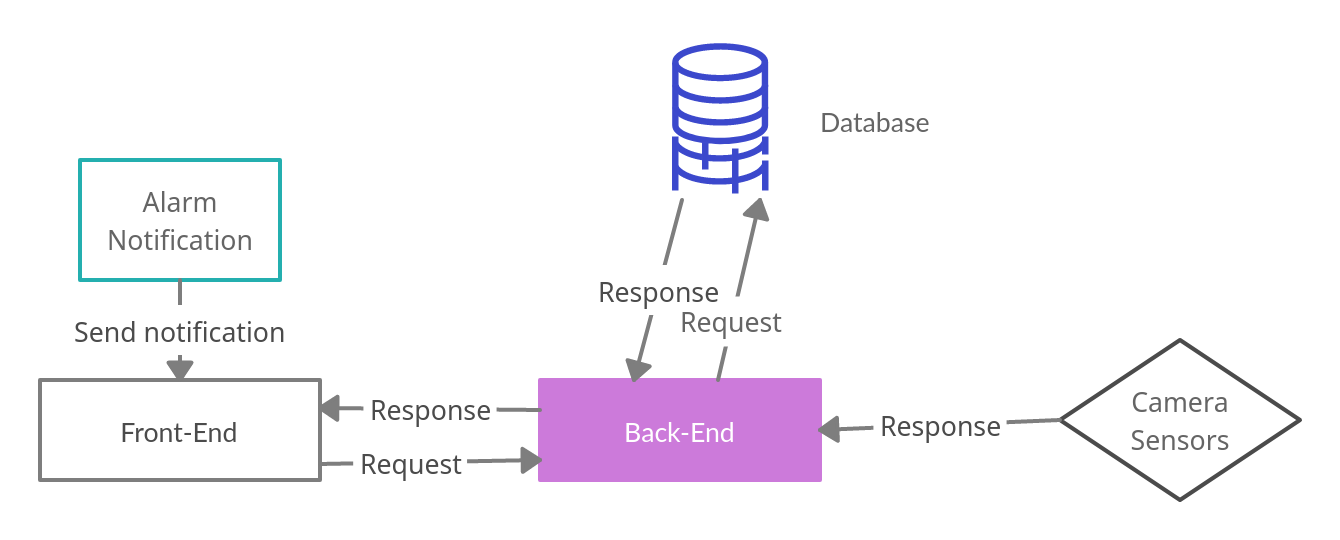
\includegraphics[scale=0.2]{Architecture.png}}
\caption{Architectural Design}
\label{fig}
\end{figure}

\emph {B. Use Cases:}\\
Each software model contains a specific set of use-cases. The use-cases give an overview about how the user will be interacting with the system. The major use-cases are shown in the Use Case diagram below:

\begin{figure}[htbp]
\centerline{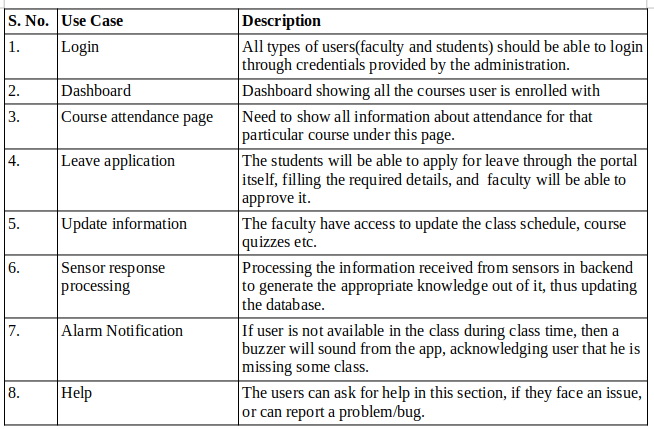
\includegraphics[scale=0.4]{Usecase.png}}
\caption{Use Cases}
\label{fig}
\end{figure}

\emph {C. User Profile diagram:}\\
A Profile diagram is any diagram created in a `profile' Package. The profile diagram shown below has all types of Users along with their Mode of Usage and Level of Familarity.\\
Below is the user profile diagram shown:\\ \\

\begin{figure}[htbp]
\centerline{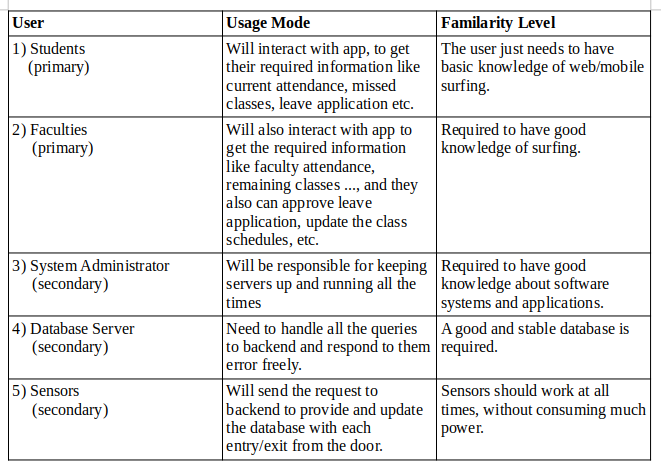
\includegraphics[scale=0.4]{Userprofile.png}}
\caption{User Profile Table}
\label{fig}
\end{figure}


\emph {D. UML Use-Case diagram:}\\
UML Use Case Diagram is shown below:

\begin{figure}[htbp]
\centerline{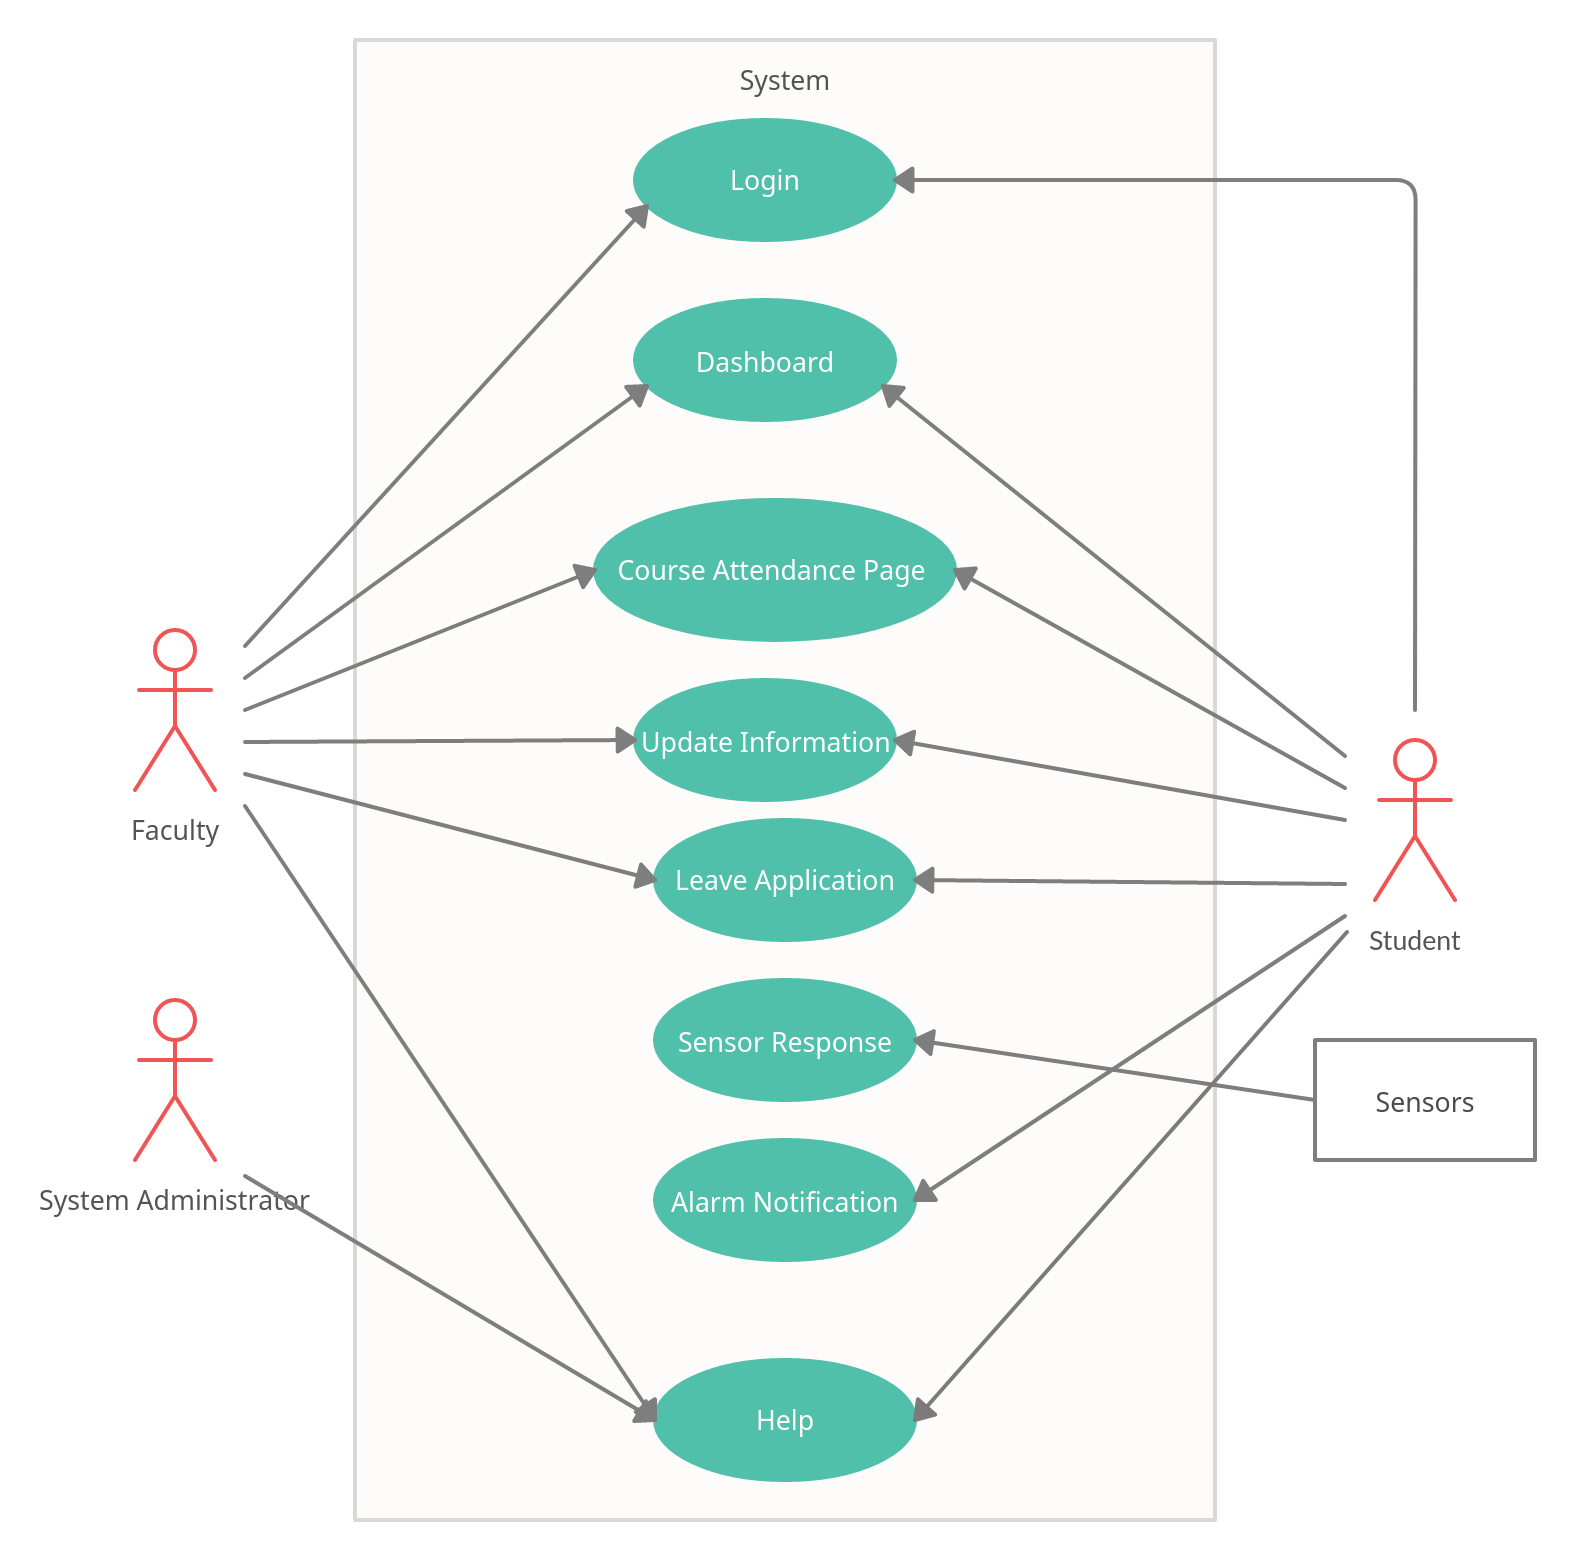
\includegraphics[scale=0.15]{UMLUsecase.png}}
\caption{UML Use-Case diagram}
\label{fig}
\end{figure}

\emph {E. UML Sequence diagram:}\\
UML Sequence Diagram is shown below:
\begin{figure}[htbp]
\centerline{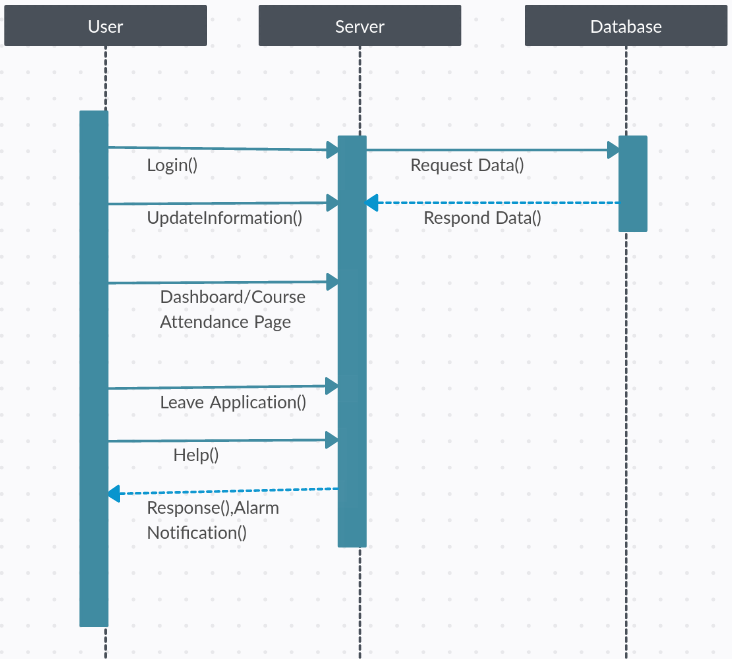
\includegraphics[scale=0.3]{UMLSequence.png}}
\caption{UML Sequence Diagram}
\label{fig}
\end{figure}\\

\emph {F. Enlisting Classes:}\\
Classes are enlisted below:
\begin{figure}[htbp]
\centerline{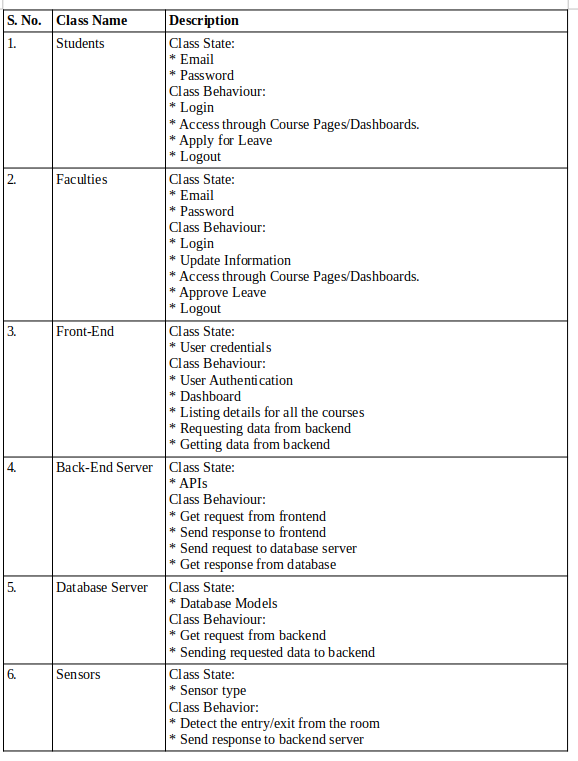
\includegraphics[scale=0.25]{Class.png}}
\caption{Enlisted Classes}
\label{fig}
\end{figure}\\

\emph {G. UML Class Diagram:}\\
The Class diagram using the enlisted classes is shown below:
\begin{figure}[htbp]
\centerline{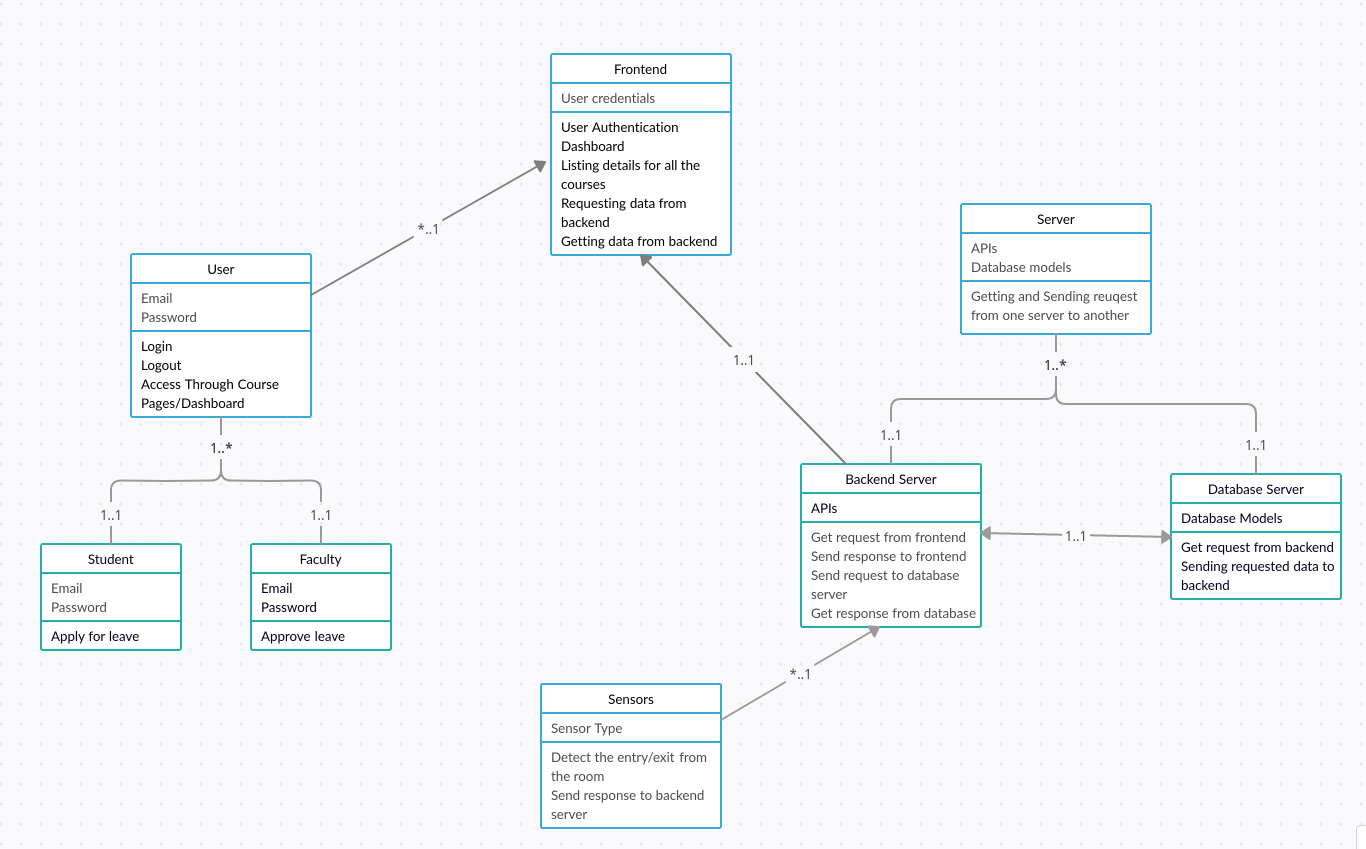
\includegraphics[scale=0.2]{ClassDiagram.png}}
\caption{UML Class Diagram}
\label{fig}
\end{figure}
\\ 
\section{Conclusion and Future Work}
Thus, in most of the institutes students need to met the threshold attendance criteria before they are allowed to sit for examinations so it becomes very important to use good attendance management in educational institutions. \\
The `Attendiiit' can be effectively used to manage attendance by not only the authorities but also the attendies as they can keep track of their attendance along with course evaluations and examinations. This prevents class strength from declining, also preventing the responsible authorities from cumbersome paper-work task.\\
The last but not the least, in future, i would like to integrate this app with the `moodle' app of our institute(IIITH). This app is responsible for all the activities associated with the courses. It lacks the information regarding the attendance, which can be fulfilled by integrating it with `Attendiiit' app, thus ripping new fruits. 

\section{References}
1. Patel UA, Swaminarayan Priya R. Development of a student attendance management system using RFID and face recognition: a review. Int J Adv Res Comput Sci Manag Stud. 2014;2(8):109–19.\\
2. Jacksi K. Design and Implementation of Online Submission And Peer Review System: A Case Study Of E-Journal Of University Of Zakho. Int J Sci Technol Res. 2015;4(8):83–5.\\
3. Jacksi K, Badiozamany S. General method for data indexing using clustering methods. Int J Sci Eng. 2015 Mar;6(3):641–4.\\
4. Jacksi K, Dimililer N, and Zeebaree SR. State of the Art Exploration Systems for Linked Data: A Review. Int J Adv Comput Sci Appl IJACSA. 2016;7(11):155–64.\\
5. Gangagowri G, Muthuselvi J, Sujitha S. Attendance Management System.\\
6. Anitha V Pai, Krishna A, Kshama PM, Correa M. Web service for student attendance management system. www.ijarse.com. 2016 Mar;5(3).\\
7. Arbain N, Nordin NF, Isa NM, Saaidin S. LAS: Web-based laboratory attendance system by integrating RFID-ARDUINO technology. In IEEE; 2014. p. 89–94.\\
8. Srinidhi M, Roy R. A web enabled secured system for attendance monitoring and real time location tracking using Biometric and Radio Frequency Identification (RFID) technology. In IEEE; 2015. p. 1–5.\\
9. Arulogun O, Olatunbosun A, Fakolujo O, Olaniyi O. RFID-based student’s attendance management system. Int J Sci Eng Res. 2013;4(2):1–9.\\
10. Kassim M, Mazlan H, Zaini N, Salleh MK. Web-based student attendance system using RFID technology. In IEEE; 2012. p. 213–8.\\
\end{document}